\documentclass[10pt]{article}
\usepackage[polish]{babel}
\usepackage[utf8]{inputenc}
\usepackage[T1]{fontenc}
\usepackage{graphicx}
\usepackage[export]{adjustbox}
\graphicspath{ {./images/} }
\usepackage{amsmath}
\usepackage{amsfonts}
\usepackage{amssymb}
\usepackage[version=4]{mhchem}
\usepackage{stmaryrd}
\usepackage{multirow}

\title{EGZAMIN MATURALNY Z MATEMATYKI POZIOM ROZSZERZONY }

\author{data: 9 maja 2016 r.\\
Godzina ROZPOCzĘCIA: 9:00\\
CZaS PRACY: \(\mathbf{1 8 0}\) minut\\
LICZBA PUNKTÓW DO UZYSKANIA: \(\mathbf{5 0}\)}
\date{}


\begin{document}
\maketitle

\includegraphics[max width=\textwidth, center]{2024_11_21_054c332d5c02f869c372g-01(1)}\\
dysleksja



\section*{Instrukcja dla zdającego}
\begin{enumerate}
  \item Sprawdź, czy arkusz egzaminacyjny zawiera 22 strony (zadania 1-16).
\end{enumerate}

Ewentualny brak zgłoś przewodniczącemu zespołu nadzorującego egzamin.\\
2. Rozwiązania zadań i odpowiedzi wpisuj w miejscu na to przeznaczonym.\\
3. Odpowiedzi do zadań zamkniętych (1-5) zaznacz na karcie odpowiedzi w części karty przeznaczonej dla zdającego. Zamaluj \(\square\) pola do tego przeznaczone. Błędne zaznaczenie otocz kółkiem \(\bigcirc_{\text {i zaznacz właściwe. }}\)\\
4. W zadaniu 6. wpisz odpowiednie cyfry w kratki pod treścią zadania.\\
5. Pamiętaj, że pominięcie argumentacji lub istotnych obliczeń w rozwiązaniu zadania otwartego (7-16) może spowodować, że za to rozwiązanie nie otrzymasz pełnej liczby punktów.\\
6. Pisz czytelnie i używaj tylko długopisu lub pióra z czarnym tuszem lub atramentem.\\
7. Nie używaj korektora, a błędne zapisy wyraźnie przekreśl.\\
8. Pamiętaj, że zapisy w brudnopisie nie będą oceniane.\\
9. Możesz korzystać z zestawu wzorów matematycznych, cyrkla i linijki oraz kalkulatora prostego.\\
10. Na tej stronie oraz na karcie odpowiedzi wpisz swój numer PESEL i przyklej naklejkę z kodem.\\
11. Nie wpisuj żadnych znaków w części przeznaczonej dla egzaminatora.\\

\includegraphics[max width=\textwidth, center]{2024_11_21_054c332d5c02f869c372g-01}

W zadaniach od 1. do 5. wybierz i zaznacz na karcie odpowiedzi poprawna odpowiedź.

\section*{Zadanie 1. (0-1)}
W rozwinięciu wyrażenia \((2 \sqrt{3} x+4 y)^{3}\) współczynnik przy iloczynie \(x y^{2}\) jest równy\\
A. \(32 \sqrt{3}\)\\
B. 48\\
C. \(96 \sqrt{3}\)\\
D. 144

\section*{Zadanie 2. (0-1)}
Wielomian \(W(x)=6 x^{3}+3 x^{2}-5 x+p\) jest podzielny przez dwumian \(x-1\) dla \(p\) równego\\
A. 4\\
B. -2\\
C. 2\\
D. -4

\section*{Zadanie 3. (0-1)}
Na rysunku przedstawiono fragment wykresu funkcji homograficznej \(y=f(x)\), której dziedziną jest zbiór \(D=(-\infty, 3) \cup(3,+\infty)\).\\
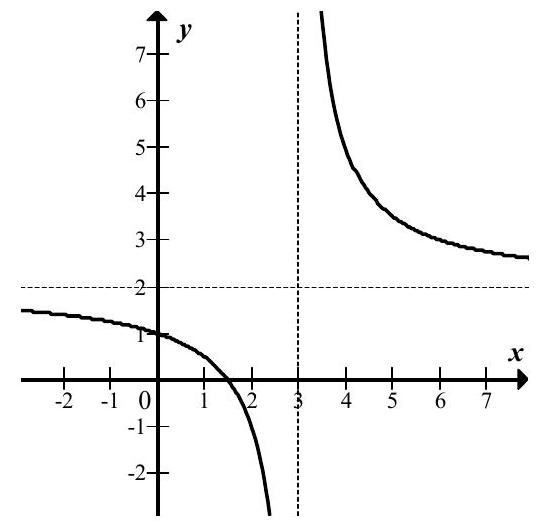
\includegraphics[max width=\textwidth, center]{2024_11_21_054c332d5c02f869c372g-02}

Równanie \(|f(x)|=p\) z niewiadomą \(x\) ma dokładnie jedno rozwiązanie\\
A. w dwóch przypadkach: \(p=0\) lub \(p=3\).\\
B. w dwóch przypadkach: \(p=0\) lub \(p=2\).\\
C. tylko wtedy, gdy \(p=3\).\\
D. tylko wtedy, gdy \(p=2\).

\section*{Zadanie 4. (0-1)}
Funkcja \(f(x)=\frac{3 x-1}{x^{2}+4}\) jest określona dla każdej liczby rzeczywistej \(x\). Pochodna tej funkcji jest określona wzorem\\
A. \(f^{\prime}(x)=\frac{-3 x^{2}+2 x+12}{\left(x^{2}+4\right)^{2}}\)\\
B. \(f^{\prime}(x)=\frac{-9 x^{2}+2 x-12}{\left(x^{2}+4\right)^{2}}\)\\
C. \(f^{\prime}(x)=\frac{3 x^{2}-2 x-12}{\left(x^{2}+4\right)^{2}}\)\\
D. \(f^{\prime}(x)=\frac{9 x^{2}-2 x+12}{\left(x^{2}+4\right)^{2}}\)

\section*{BRUDNOPIS (nie podlega ocenie)}
\begin{center}

\includegraphics[max width=\textwidth]{2024_11_21_054c332d5c02f869c372g-03}
\end{center}

\section*{Zadanie 5. (0-1)}
Granica \(\lim _{n \rightarrow \infty} \frac{\left(p n^{2}+4 n\right)^{3}}{5 n^{6}-4}=-\frac{8}{5}\). Wynika stąd, że\\
A. \(\quad p=-8\)\\
B. \(p=4\)\\
C. \(p=2\)\\
D. \(p=-2\)

\section*{Zadanie 6. (0-2)}
Wśród 10 tysięcy mieszkańców pewnego miasta przeprowadzono sondaż dotyczący budowy przedszkola publicznego. Wyniki sondażu przedstawiono w tabeli.

\begin{center}
\begin{tabular}{|l|c|c|}
\hline
Badane grupy & \begin{tabular}{c}
Liczba osób popierających \\
budowę przedszkola \\
\end{tabular} & \begin{tabular}{c}
Liczba osób niepopierających \\
budowy przedszkola \\
\end{tabular} \\
\hline
Kobiety & 5140 & 1860 \\
\hline
Mężczyźni & 2260 & 740 \\
\hline
\end{tabular}
\end{center}

Oblicz prawdopodobieństwo zdarzenia polegającego na tym, że losowo wybrana osoba, spośród ankietowanych, popiera budowę przedszkola, jeśli wiadomo, że jest mężczyzną. Zakoduj trzy pierwsze cyfry po przecinku nieskończonego rozwinięcia dziesiętnego otrzymanego wyniku.\\

\includegraphics[max width=\textwidth, center]{2024_11_21_054c332d5c02f869c372g-04}

\section*{BRUDNOPIS (nie podlega ocenie)}
\begin{center}

\includegraphics[max width=\textwidth]{2024_11_21_054c332d5c02f869c372g-04(1)}
\end{center}

\section*{Zadanie 7. (0-2)}
Dany jest ciąg geometryczny \(\left(a_{n}\right)\) określony wzorem \(a_{n}=\left(\frac{1}{2 x-371}\right)^{n}\) dla \(n \geq 1\). Wszystkie wyrazy tego ciągu są dodatnie. Wyznacz najmniejszą liczbę całkowitą \(x\), dla której nieskończony szereg \(a_{1}+a_{2}+a_{3}+\ldots\) jest zbieżny.\\

\includegraphics[max width=\textwidth, center]{2024_11_21_054c332d5c02f869c372g-05}

Odpowiedź:

\begin{center}
\begin{tabular}{|c|l|c|c|}
\hline
\multirow{2}{*}{\begin{tabular}{c}
Wypełnia \\
egzaminator \\
\end{tabular}} & Nr zadania & \(\mathbf{6 .}\) & \(\mathbf{7 .}\) \\
\cline { 2 - 4 }
 & Maks. liczba pkt & \(\mathbf{2}\) & \(\mathbf{2}\) \\
\cline { 2 - 4 }
 & Uzyskana liczba pkt &  &  \\
\hline
\end{tabular}
\end{center}

\section*{Zadanie 8. (0-3)}
Wykaż, że dla dowolnych dodatnich liczb rzeczywistych \(x\) i \(y\) takich, że \(x^{2}+y^{2}=2\), prawdziwa jest nierówność \(x+y \leq 2\).\\

\includegraphics[max width=\textwidth, center]{2024_11_21_054c332d5c02f869c372g-06}

\begin{center}
\begin{tabular}{|c|l|c|}
\hline
\multirow{2}{*}{\begin{tabular}{l}
Wypelnia \\
egzaminator \\
\end{tabular}} & Nr zadania & 8. \\
\cline { 2 - 3 }
 & Maks. liczba pkt & 3 \\
\cline { 2 - 3 }
 & Uzyskana liczba pkt &  \\
\hline
\end{tabular}
\end{center}

\section*{Zadanie 9. (0-3)}
Dany jest prostokąt \(A B C D\). Okrąg wpisany w trójkąt \(B C D\) jest styczny do przekątnej \(B D\) w punkcie \(N\). Okrąg wpisany w trójkąt \(A B D\) jest styczny do boku \(A D\) w punkcie \(M\), a środek \(S\) tego okręgu leży na odcinku \(M N\), jak na rysunku.\\
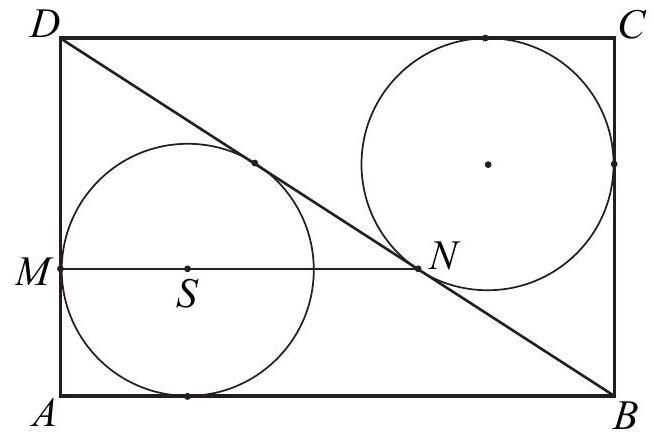
\includegraphics[max width=\textwidth, center]{2024_11_21_054c332d5c02f869c372g-08}

Wykaż, że \(|M N|=|A D|\).\\

\includegraphics[max width=\textwidth, center]{2024_11_21_054c332d5c02f869c372g-08(1)}\\

\includegraphics[max width=\textwidth, center]{2024_11_21_054c332d5c02f869c372g-09}

\section*{Zadanie 10. (0-4)}
Wyznacz wszystkie wartości parametru \(a\), dla których wykresy funkcji \(f\) i \(g\), określonych wzorami \(f(x)=x-2\) oraz \(g(x)=5-a x\), przecinają się w punkcie o obu współzzędnych dodatnich.\\

\includegraphics[max width=\textwidth, center]{2024_11_21_054c332d5c02f869c372g-10}

Odpowiedź: \(\qquad\)

\section*{Zadanie 11. (0-4)}
Rozwiąż nierówność \(\frac{2 \cos x-\sqrt{3}}{\cos ^{2} x}<0\) w przedziale \(\langle 0,2 \pi\rangle\).\\

\includegraphics[max width=\textwidth, center]{2024_11_21_054c332d5c02f869c372g-11}

Odpowiedź: \(\qquad\)

\begin{center}
\begin{tabular}{|c|l|c|c|}
\hline
\multirow{2}{*}{\begin{tabular}{c}
Wypelnia \\
egzaminator \\
\end{tabular}} & Nr zadania & 10. & 11. \\
\cline { 2 - 4 }
 & Maks. liczba pkt & 4 & 4 \\
\cline { 2 - 4 }
 & Uzyskana liczba pkt &  &  \\
\hline
\end{tabular}
\end{center}

\section*{Zadanie 12. (0-6)}
Dany jest trójmian kwadratowy \(f(x)=x^{2}+2(m+1) x+6 m+1\). Wyznacz wszystkie rzeczywiste wartości parametru \(m\), dla których ten trójmian ma dwa różne pierwiastki \(x_{1}, x_{2}\) tego samego znaku, spełniające warunek \(\left|x_{1}-x_{2}\right|<3\).\\

\includegraphics[max width=\textwidth, center]{2024_11_21_054c332d5c02f869c372g-12}\\

\includegraphics[max width=\textwidth, center]{2024_11_21_054c332d5c02f869c372g-13}

Odpowiedź: \(\qquad\)

\begin{center}
\begin{tabular}{|c|l|c|}
\hline
\multirow{2}{*}{\begin{tabular}{c}
Wypelnia \\
egzaminator \\
\end{tabular}} & Nr zadania & 12. \\
\cline { 2 - 3 }
 & Maks. liczba pkt & \(\mathbf{6}\) \\
\cline { 2 - 3 }
 & Uzyskana liczba pkt &  \\
\hline
\end{tabular}
\end{center}

\section*{Zadanie 13. (0-5)}
Punkty \(A=(30,32)\) i \(B=(0,8)\) są sąsiednimi wierzchołkami czworokąta \(A B C D\) wpisanego w okrąg. Prosta o równaniu \(x-y+2=0\) jest jedyną osią symetrii tego czworokąta i zawiera przekątną \(A C\). Oblicz współrzędne wierzchołków \(C\) i \(D\) tego czworokąta.\\

\includegraphics[max width=\textwidth, center]{2024_11_21_054c332d5c02f869c372g-14}\\

\includegraphics[max width=\textwidth, center]{2024_11_21_054c332d5c02f869c372g-15}

Odpowiedź: \(\qquad\)

\begin{center}
\begin{tabular}{|c|l|c|}
\hline
\multirow{2}{*}{\begin{tabular}{c}
Wypelnia \\
egzaminator \\
\end{tabular}} & Nr zadania & 13. \\
\cline { 2 - 3 }
 & Maks. liczba pkt & \(\mathbf{5}\) \\
\cline { 2 - 3 }
 & Uzyskana liczba pkt &  \\
\hline
\end{tabular}
\end{center}

\section*{Zadanie 14. (0-3)}
Rozpatrujemy wszystkie liczby naturalne dziesięciocyfrowe, w zapisie których mogą występować wyłącznie cyfry \(1,2,3\), przy czym cyfra 1 występuje dokładnie trzy razy. Uzasadnij, że takich liczb jest 15360.\\

\includegraphics[max width=\textwidth, center]{2024_11_21_054c332d5c02f869c372g-16}\\

\includegraphics[max width=\textwidth, center]{2024_11_21_054c332d5c02f869c372g-17}

Odpowiedź: \(\qquad\)

\begin{center}
\begin{tabular}{|c|l|c|}
\hline
\multirow{2}{*}{\begin{tabular}{c}
Wypelnia \\
egzaminator \\
\end{tabular}} & Nr zadania & 14. \\
\cline { 2 - 3 }
 & Maks. liczba pkt & 3 \\
\cline { 2 - 3 }
 & Uzyskana liczba pkt &  \\
\hline
\end{tabular}
\end{center}

\section*{Zadanie 15. (0-6)}
W ostrosłupie prawidłowym czworokątnym \(A B C D S\) o podstawie \(A B C D\) wysokość jest równa 5, a kąt między sąsiednimi ścianami bocznymi ostrosłupa ma miarę \(120^{\circ}\). Oblicz objętość tego ostrosłupa.\\

\includegraphics[max width=\textwidth, center]{2024_11_21_054c332d5c02f869c372g-18}\\

\includegraphics[max width=\textwidth, center]{2024_11_21_054c332d5c02f869c372g-19}

Odpowiedź: \(\qquad\)

\begin{center}
\begin{tabular}{|c|l|c|}
\hline
\multirow{2}{*}{\begin{tabular}{c}
Wypelnia \\
egzaminator \\
\end{tabular}} & Nr zadania & 15. \\
\cline { 2 - 3 }
 & Maks. liczba pkt & 6 \\
\cline { 2 - 3 }
 & Uzyskana liczba pkt &  \\
\hline
\end{tabular}
\end{center}

\section*{Zadanie 16. (0-7)}
Parabola o równaniu \(y=2-\frac{1}{2} x^{2}\) przecina oś \(O x\) układu współrzędnych w punktach \(A=(-2,0)\) i \(B=(2,0)\). Rozpatrujemy wszystkie trapezy równoramienne \(A B C D\), których dłuższą podstawą jest odcinek \(A B\), a końce \(C\) i \(D\) krótszej podstawy leżą na paraboli (zobacz rysunek).\\
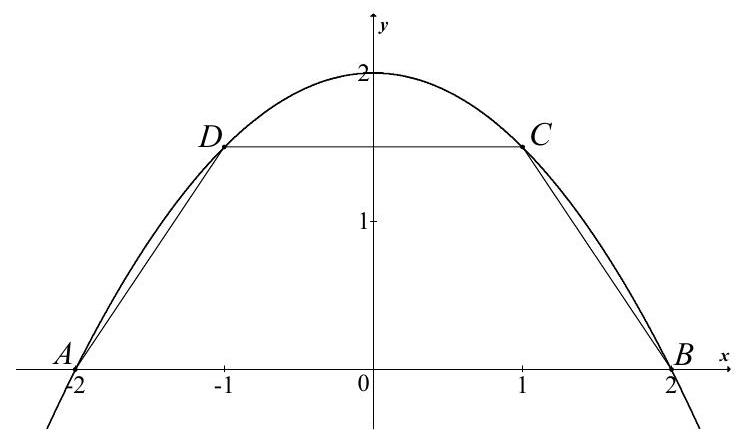
\includegraphics[max width=\textwidth, center]{2024_11_21_054c332d5c02f869c372g-20}

Wyznacz pole trapezu \(A B C D\) w zależności od pierwszej współrzędnej wierzchołka \(C\). Oblicz współrzędne wierzchołka \(C\) tego z rozpatrywanych trapezów, którego pole jest największe.

\begin{center}
\begin{tabular}{|c|c|c|c|c|c|c|c|c|c|c|c|c|c|c|c|c|c|c|c|c|c|c|c|c|c|}
\hline
 &  &  &  &  &  &  &  &  &  &  &  &  &  &  &  &  &  &  &  &  &  &  &  &  &  \\
\hline
 &  &  &  &  &  &  &  &  &  &  &  &  &  &  &  &  &  &  &  &  &  &  &  &  &  \\
\hline
 &  &  &  &  &  &  &  &  &  &  &  &  &  &  &  &  &  &  &  &  &  &  &  &  &  \\
\hline
 &  &  &  &  &  &  &  &  &  &  &  &  &  &  &  &  &  &  &  &  &  &  &  &  &  \\
\hline
 &  &  &  &  &  &  &  &  &  &  &  &  &  &  &  &  &  &  &  &  &  &  &  &  &  \\
\hline
 &  &  &  &  &  &  &  &  &  &  &  &  &  &  &  &  &  &  &  &  &  &  &  &  &  \\
\hline
 &  &  &  &  &  &  &  &  &  &  &  &  &  &  &  &  &  &  &  &  &  &  &  &  &  \\
\hline
 &  &  &  &  &  &  &  &  &  &  &  &  &  &  &  &  &  &  &  &  &  &  &  &  &  \\
\hline
 &  &  &  &  &  &  &  &  &  &  &  &  &  &  &  &  &  &  &  &  &  &  &  &  &  \\
\hline
 &  &  &  &  &  &  &  &  &  &  &  &  &  &  &  &  &  &  &  &  &  &  &  &  &  \\
\hline
 &  &  &  &  &  &  &  &  &  &  &  &  &  &  &  &  &  &  &  &  &  &  &  &  &  \\
\hline
 &  &  &  &  &  &  &  &  &  &  &  &  &  &  &  &  &  &  &  &  &  &  &  &  &  \\
\hline
 &  &  &  &  &  &  &  &  &  &  &  &  &  &  &  &  &  &  &  &  &  &  &  &  &  \\
\hline
 &  &  &  &  &  &  &  &  &  &  &  &  &  &  &  &  &  &  &  &  &  &  &  &  &  \\
\hline
 &  &  &  &  &  &  &  &  &  &  &  &  &  &  &  &  &  &  &  &  &  &  &  &  &  \\
\hline
 &  &  &  &  &  &  &  &  &  &  &  &  &  &  &  &  &  &  &  &  &  &  &  &  &  \\
\hline
 &  &  &  &  &  &  &  &  &  &  &  &  &  &  &  &  &  &  &  &  &  &  &  &  &  \\
\hline
 &  &  &  &  &  &  &  &  &  &  &  &  &  &  &  &  &  &  &  &  &  &  &  &  &  \\
\hline
 &  &  &  &  &  &  &  &  &  &  &  &  &  &  &  &  &  &  &  &  &  &  &  &  &  \\
\hline
 &  &  &  &  &  &  &  &  &  &  &  &  &  &  &  &  &  &  &  &  &  &  &  &  &  \\
\hline
 &  &  &  &  &  &  &  &  &  &  &  &  &  &  &  &  &  &  &  &  &  &  &  &  &  \\
\hline
 &  &  &  &  &  &  &  &  &  &  &  &  &  &  &  &  &  &  &  &  &  &  &  &  &  \\
\hline
 &  &  &  &  &  &  &  &  &  &  &  &  &  &  &  &  &  &  &  &  &  &  &  &  &  \\
\hline
 &  &  &  &  &  &  &  &  &  &  &  &  &  &  &  &  &  &  &  &  &  &  &  &  &  \\
\hline
 &  &  &  &  &  &  &  &  &  &  &  &  &  &  &  &  &  &  &  &  &  &  &  &  &  \\
\hline
 &  &  &  &  &  &  &  &  &  &  &  &  &  &  &  &  &  &  &  &  &  &  &  &  &  \\
\hline
 &  &  &  &  &  &  &  &  &  &  &  &  &  &  &  &  &  &  &  &  &  &  &  &  &  \\
\hline
 &  &  &  &  &  &  &  &  &  &  &  &  &  &  &  &  &  &  &  &  &  &  &  &  &  \\
\hline
 &  &  &  &  &  &  &  &  &  &  &  &  &  &  &  &  &  &  &  &  &  &  &  &  &  \\
\hline
 &  &  &  &  &  &  &  &  &  &  &  &  &  &  &  &  &  &  &  &  &  &  &  &  &  \\
\hline
 &  &  &  &  &  &  &  &  &  &  &  &  &  &  &  &  &  &  &  &  &  &  &  &  &  \\
\hline
 &  &  &  &  &  &  &  &  &  &  &  &  &  &  &  &  &  &  &  &  &  &  &  &  &  \\
\hline
\end{tabular}
\end{center}

\begin{center}

\includegraphics[max width=\textwidth]{2024_11_21_054c332d5c02f869c372g-21}
\end{center}

Odpowiedź: \(\qquad\)

\begin{center}
\begin{tabular}{|c|l|c|}
\hline
\multirow{2}{*}{\begin{tabular}{c}
Wypelnia \\
egzaminator \\
\end{tabular}} & Nr zadania & 16. \\
\cline { 2 - 3 }
 & Maks. liczba pkt & 7 \\
\cline { 2 - 3 }
 & Uzyskana liczba pkt &  \\
\hline
\end{tabular}
\end{center}

\section*{BRUDNOPIS (nie podlega ocenie)}

\end{document}